\section{Environments with Homogeneous Agents}
\subsection{Homogeneous Agents}

% Colors used across this section
\definecolor{cardfill}{RGB}{252,244,214}
\definecolor{cardborder}{RGB}{120,110,80}
\definecolor{seacown}{RGB}{0,102,153}      % own on-policy experience
\definecolor{seacshared}{RGB}{204,85,0}    % shared, IS-corrected experience

% Put this BEFORE \begin{frame} — in the preamble if you'll reuse it elsewhere,
% or just above the frame if it's only used once.
\newcommand{\drawnetwork}[4]{%
    \begin{scope}[shift={(#1,#2)}, scale=#3]

        % Input layer
        \foreach \y/\i in {1.2/1,0.4/2,-0.4/3,-1.2/4}
            \node[neuron] (#4-in-\i) at (0,\y) {};

        % First hidden layer
        \foreach \y/\i in {1.5/1,0.75/2,0/3,-0.75/4,-1.5/5}
            \node[neuron] (#4-hone-\i) at (1.1,\y) {};

        % Second hidden layer
        \foreach \y/\i in {1.5/1,0.75/2,0/3,-0.75/4,-1.5/5}
            \node[neuron] (#4-htwo-\i) at (2.2,\y) {};

        % Output layer
        \foreach \y/\i in {0.9/1,0.3/2,-0.3/3,-0.9/4}
            \node[neuron] (#4-out-\i) at (3.3,\y) {};

        % Fully connected edges
        \foreach \i in {1,...,4}
            \foreach \j in {1,...,5}
                \draw[connection] (#4-in-\i) -- (#4-hone-\j);

        \foreach \i in {1,...,5}
            \foreach \j in {1,...,5}
                \draw[connection] (#4-hone-\i) -- (#4-htwo-\j);

        \foreach \i in {1,...,5}
            \foreach \j in {1,...,4}
                \draw[connection] (#4-htwo-\i) -- (#4-out-\j);

    \end{scope}
}

% Reusable sketch styles for the agent/location illustrations
\tikzset{
    location/.style={
        rectangle, draw=black, thick,
        minimum width=0.8cm, minimum height=0.8cm
    },
    agentred/.style={
        circle, draw=black, thick, fill=red!60,
        minimum size=0.65cm
    },
    agentblue/.style={
        circle, draw=black, thick, fill=blue!35,
        minimum size=0.65cm
    },
    agentdart/.style={
        dart, draw=violet!80!black, fill=violet!35, thick,
        minimum size=0.75cm
    },
    agenttriangle/.style={
        isosceles triangle, isosceles triangle apex angle=60,
        draw=teal!70!black, fill=teal!35, thick,
        minimum size=0.75cm
    },
    move/.style={
        ->, thick, dashed, bend left=20, >=Latex
    }
}

\begin{frame}
\frametitle{Homogeneous agents: Motivation}

Previously, we have seen environments and agents in which we have used independent learning algorithms such as DQN. Problem? The huge number of parameters and the slow training process.

\vspace{0.5em}

\centering
\begin{adjustbox}{max width=0.8\linewidth, max height=0.7\textheight}
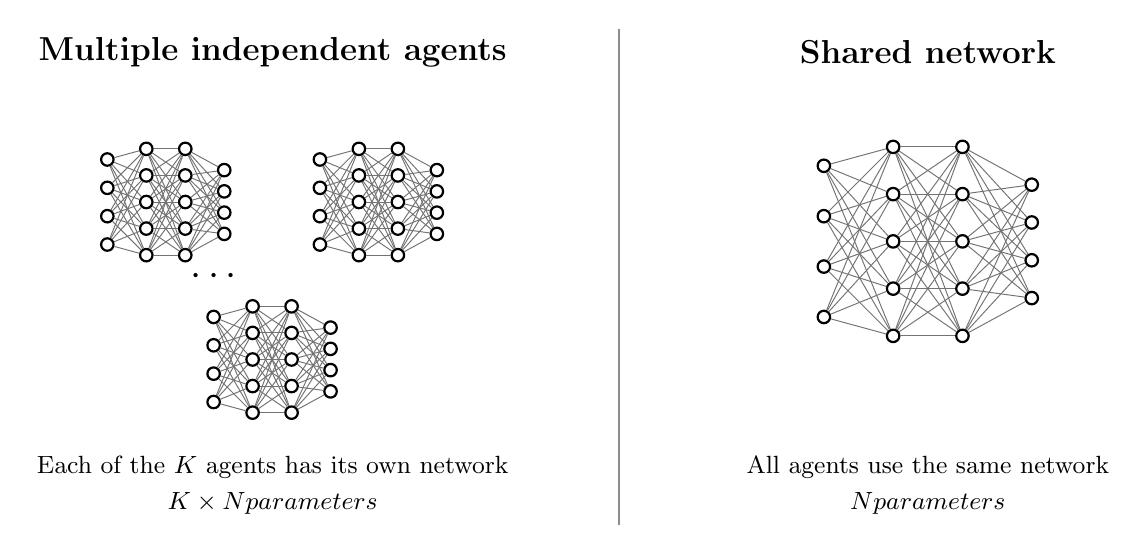
\begin{tikzpicture}[
    neuron/.style={
        circle,
        draw,
        thick,
        minimum size=4.5pt,
        inner sep=0pt
    },
    connection/.style={
        draw=black!55,
        line width=0.35pt
    },
    networkbox/.style={
        draw=black!25,
        rounded corners,
        inner sep=5pt
    },
    title/.style={
        font=\bfseries\large
    },
    explanation/.style={
        align=center,
        font=\small
    }
]

% =========================================================
% Divider
% =========================================================
\draw[thick, black!45] (0,-3.1) -- (0,3.2);

% =========================================================
% LEFT: multiple independent networks
% =========================================================
\node[title] at (-4.4,2.9) {Multiple independent agents};

\drawnetwork{-6.5}{1.0}{0.45}{agentone}
\drawnetwork{-3.8}{1.0}{0.45}{agenttwo}
\drawnetwork{-5.15}{-1.0}{0.45}{agentthree}

\node[font=\Large] at (-5.15,0.05) {$\cdots$};

\node[explanation] at (-4.4,-2.6) {
    Each of the $K$ agents has its own network\\[2pt]
    $K \times N \text{ parameters}$
};

% =========================================================
% RIGHT: one shared network
% =========================================================
\node[title] at (3.92,2.9) {Shared network};

\drawnetwork{2.6}{0.5}{0.8}{shared}

% Multiple agent inputs
% \node (input1) at (1.0,1.5) {$h_1^t$};
% \node (input2) at (1.0,0.5) {$h_i^t$};
% \node (input3) at (1.0,-0.5) {$h_K^t$};

% \draw[-{Latex}, thick] (input1) -- (shared-in-1);
% \draw[-{Latex}, thick] (input2) -- (shared-in-2);
% \draw[-{Latex}, thick] (input3) -- (shared-in-4);

\node[explanation] at (3.92,-2.6) {
    All agents use the same network\\[2pt]
    $N \text{ parameters}$
};

\end{tikzpicture}%
\end{adjustbox}

\end{frame}

\begin{frame}
    \frametitle{Homogeneous Agents: Motivation}

    \begin{columns}[T,onlytextwidth]
    % Left column
        \begin{column}{0.48\textwidth}
            \centering
            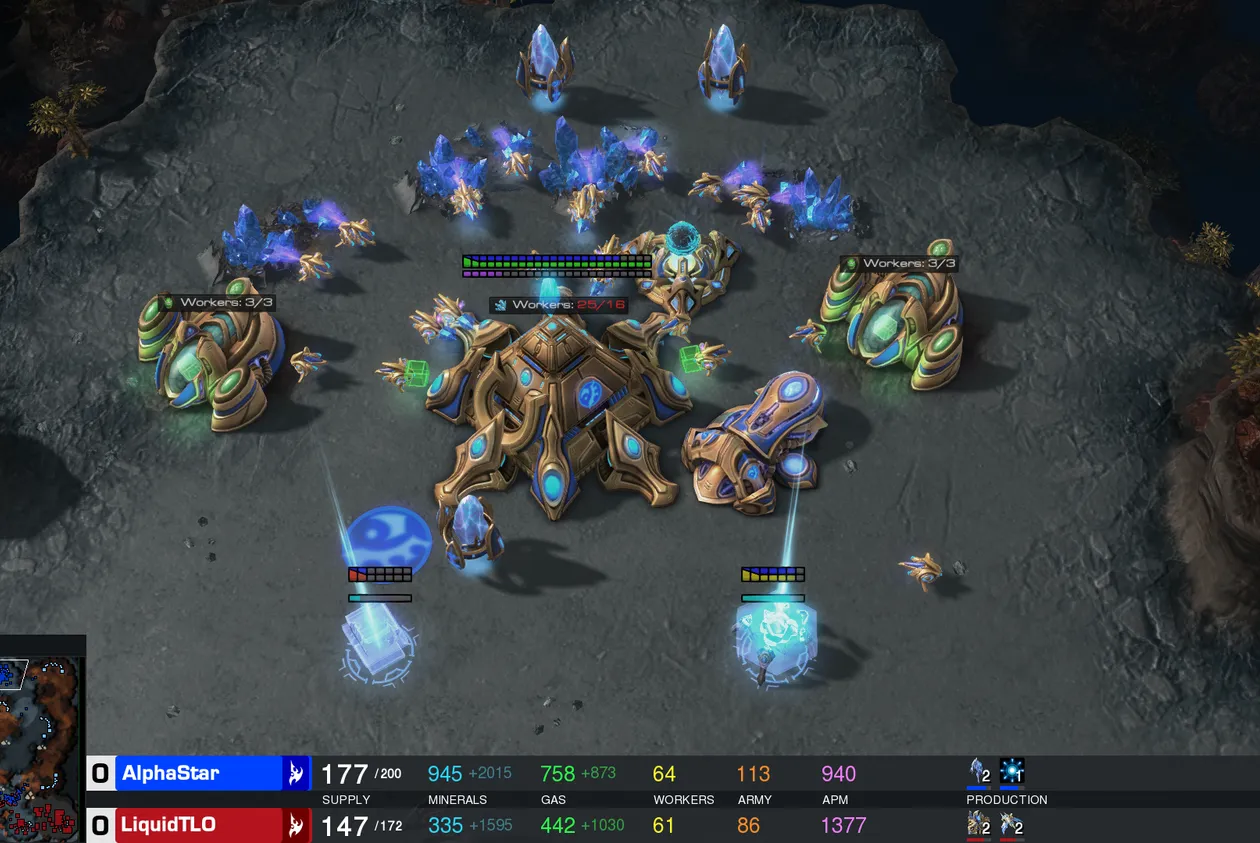
\includegraphics[
                width=\linewidth,
                height=0.55\textheight,
                keepaspectratio
            ]{media/starcraft.png}\par
            \vspace{0.4em}
            {\small \textbf{Starcraft:} a game with Agents with different roles, and usually different goals}
        \end{column}

        \hfill
    % Right column
        \begin{column}{0.48\textwidth}
        \centering
        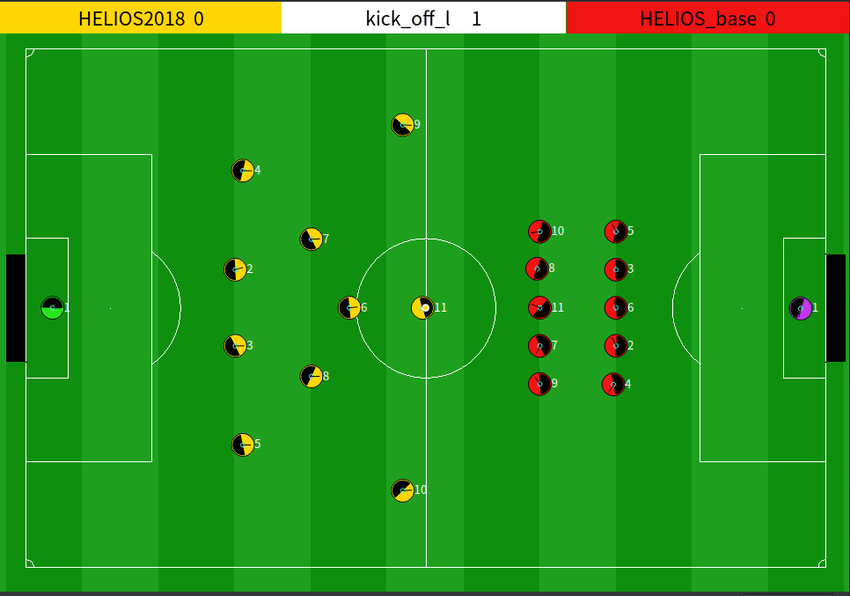
\includegraphics[
            width=\linewidth,
            height=0.55\textheight,
            keepaspectratio
        ]{media/robocup_simulation_helios.png}\par
        \vspace{0.4em}
        {\small \textbf{Robocup Simulation:} The agents have the same action space, same goals and observation abilities, and are interchangeable}
        \end{column}
    \end{columns}
\end{frame}

% =========================================================
% (1) Weakly homogeneous agents: definition | sketch
% =========================================================
\begin{frame}
\frametitle{Weakly Homogeneous Agents}

\begin{columns}[T,onlytextwidth]

% ---------- LEFT: definition ----------
\begin{column}{0.56\textwidth}
\begin{block}{Definition: Weakly homogeneous agents}
\small
An environment has weakly homogeneous agents if for any joint policy
$\pi = (\pi_1, \pi_2, \ldots, \pi_n)$
and permutation between agents $\sigma : I \to I$, the following holds:
\begin{center}
\adjustbox{max width=0.96\linewidth}{%
\colorbox{blue!20}{$
\displaystyle
U_i(\pi)
=
U_{\sigma(i)}
\left(
\left\langle
\pi_{\sigma(1)}, \pi_{\sigma(2)}, \ldots, \pi_{\sigma(n)}
\right\rangle
\right),
\quad
\forall i \in I
$}}
\end{center}
\end{block}

\vspace{0.6em}
{\small
\textbf{Intuition:} agents can \emph{swap} their policies without changing
the expected returns --- the agents are interchangeable.
}
\end{column}

% ---------- RIGHT: sketch ----------
\begin{column}{0.4\textwidth}
\centering
\resizebox{0.9\linewidth}{!}{%
\begin{tikzpicture}
\useasboundingbox (-1.0,-2.3) rectangle (4.1,2.3);

\node[location] (a1) at (0,0) {};
\node[location] (a2) at (3.1,0) {};

\node[agentred]  (r1) at (0,1.2) {};
\node[agentblue] (b1) at (3.1,-1.2) {};

\draw[move] (r1.east) to (a2.north);
\draw[move] (b1.west) to (a1.south);
\end{tikzpicture}%
}

\vspace{0.4em}
{\small Agents have to move to two \emph{different} locations.}
\end{column}

\end{columns}

\end{frame}

% =========================================================
% (2) Strongly homogeneous agents: definition | sketch
% =========================================================
\begin{frame}
\frametitle{Strongly Homogeneous Agents}
\framesubtitle{But what if agents are weakly homogeneous and even the goals are the same?}

\begin{columns}[T,onlytextwidth]

% ---------- LEFT: definition ----------
\begin{column}{0.56\textwidth}
\begin{block}{Definition: Strongly homogeneous agents}
\small
An environment has strongly homogeneous agents if the optimal joint policy
consists of identical individual policies, formally:
\begin{itemize}
    \item The environment has weakly homogeneous agents.
    \item The optimal joint policy
    $\pi^{*} = (\pi_1, \pi_2, \ldots, \pi_n)$
    consists of identical policies
    \colorbox{blue!20}{$\pi_1 = \pi_2 = \cdots = \pi_n$}
\end{itemize}
\end{block}

\vspace{0.3em}
{\small
\textbf{Intuition:} not only are the agents interchangeable --- at the
optimum they all \emph{behave identically}.
}
\end{column}

% ---------- RIGHT: sketch ----------
\begin{column}{0.4\textwidth}
\centering
\vspace{0.3em}
\resizebox{0.72\linewidth}{!}{%
\begin{tikzpicture}
\useasboundingbox (-1.0,-2.3) rectangle (4.1,2.3);

\node[location] (a3) at (1.55,0) {};

\node[agentred]  (r2) at (0,1.3) {};
\node[agentblue] (b2) at (3.1,-1.3) {};

\draw[move] (r2.east) to (a3.north);
\draw[move] (b2.west) to (a3.south);
\end{tikzpicture}%
}

\vspace{0.2em}
{\small Both agents have to move to the \emph{same} location.}
\end{column}

\end{columns}

\end{frame}

% =========================================================
% (3) Three-column comparison, cleaned up
% =========================================================
\begin{frame}
\frametitle{Homogeneous vs. Non-Homogeneous Agents}

\begin{columns}[T,onlytextwidth]

% =====================================================
% Column 1: weakly homogeneous
% =====================================================
\begin{column}{0.32\textwidth}
\centering

\adjustbox{max width=0.95\linewidth, max height=0.36\textheight}{%
\begin{tikzpicture}
\useasboundingbox (-1.0,-2.4) rectangle (4.1,2.4);

\node[location] (a1) at (0,0) {};
\node[location] (a2) at (3.1,0) {};

\node[agentred]  (r1) at (0,1.2) {};
\node[agentblue] (b1) at (3.1,-1.2) {};

\draw[move] (r1.east) to (a2.north);
\draw[move] (b1.west) to (a1.south);
\end{tikzpicture}%
}

\vspace{0.3em}
\begin{minipage}[t][1.9cm][t]{\linewidth}
\centering
\small
\textbf{(a) Weakly homogeneous agents}

\vspace{0.3em}
Agents are interchangeable, but must move to different locations.
\end{minipage}

\end{column}
\hfill
% =====================================================
% Column 2: strongly homogeneous
% =====================================================
\begin{column}{0.32\textwidth}
\centering

\adjustbox{max width=0.95\linewidth, max height=0.36\textheight}{%
\begin{tikzpicture}
\useasboundingbox (-1.0,-2.4) rectangle (4.1,2.4);

\node[location] (a3) at (1.55,0) {};

\node[agentred]  (r2) at (0,1.3) {};
\node[agentblue] (b2) at (3.1,-1.3) {};

\draw[move] (r2.east) to (a3.north);
\draw[move] (b2.west) to (a3.south);
\end{tikzpicture}%
}

\vspace{0.3em}
\begin{minipage}[t][1.9cm][t]{\linewidth}
\centering
\small
\textbf{(b) Strongly homogeneous agents}

\vspace{0.3em}
Both agents can move to the same location.
\end{minipage}

\end{column}
\hfill
% =====================================================
% Column 3: non-homogeneous
% =====================================================
\begin{column}{0.32\textwidth}
\centering

\adjustbox{max width=0.95\linewidth, max height=0.36\textheight}{%
\begin{tikzpicture}
\useasboundingbox (-1.0,-2.4) rectangle (4.1,2.4);

\node[agentdart]     (a4) at (0,1.9) {};
\node[agenttriangle] (a5) at (3.1,-1.9) {};

\node[location] (t1) at (0,0) {};
\node[location] (t2) at (3.1,0) {};

\draw[move] (a4.east) to (t1.north);
\draw[move] (a5.west) to (t2.south);
\end{tikzpicture}%
}

\vspace{0.3em}
\begin{minipage}[t][1.9cm][t]{\linewidth}
\centering
\small
\textbf{(c) Non-homogeneous agents}

\vspace{0.3em}
Agents are inherently different: different roles, capabilities, or action spaces.
\end{minipage}

\end{column}

\end{columns}

\centering
But if we have homogeneity, how can we use this for our gain?

\end{frame}

% Subsection --- Parameter sharing
\subsection{Parameter Sharing}
\begin{frame}
    \frametitle{Parameter sharing}
    When having strongly homogeneous agents, we know that all agents use identical policies. So do we need to keep different parameters for each? Answer is NO
    \centering
\begin{adjustbox}{max width=0.95\textwidth,max height=0.6\textheight}
\begin{tikzpicture}[
    >=Latex,
    every node/.style={font=\large},
    input/.style={
        font=\large,
        inner sep=1pt
    },
    valuebox/.style={
        draw=green!55!black,
        fill=green!15,
        very thick,
        rounded corners=4pt,
        minimum width=2.3cm,
        minimum height=0.8cm,
        align=center
    },
    policybox/.style={
        draw=orange!85!black,
        fill=orange!15,
        very thick,
        rounded corners=4pt,
        minimum width=2.3cm,
        minimum height=0.8cm,
        align=center
    },
    arrow/.style={
        ->,
        thick
    }
]

% =====================================================
% Left side: separate value networks
% =====================================================
\node[input] (h1v) at (0,3.3) {$h_1^t$};
\node[input] (dotsv) at (0,2.2) {$\vdots$};
\node[input] (hnv) at (0,1.1) {$h_n^t$};

\node[valuebox] (v1) at (2.6,3.3) {$V(\cdot;\theta_1)$};
\node[valuebox] (v2) at (2.6,2.2) {$\vdots$};
\node[valuebox] (vn) at (2.6,1.1) {$V(\cdot;\theta_n)$};

\draw[arrow] (h1v) -- (v1.west);
\draw[arrow] (dotsv) -- (v2.west);
\draw[arrow] (hnv) -- (vn.west);

% =====================================================
% Left side: separate policy networks
% =====================================================
\node[input] (h1p) at (0,-0.6) {$h_1^t$};
\node[input] (dotsp) at (0,-1.7) {$\vdots$};
\node[input] (hnp) at (0,-2.8) {$h_n^t$};

\node[policybox] (p1) at (2.6,-0.6) {$\pi(\cdot;\phi_1)$};
\node[policybox] (p2) at (2.6,-1.7) {$\vdots$};
\node[policybox] (pn) at (2.6,-2.8) {$\pi(\cdot;\phi_n)$};

\draw[arrow] (h1p) -- (p1.west);
\draw[arrow] (dotsp) -- (p2.west);
\draw[arrow] (hnp) -- (pn.west);

% =====================================================
% Right side: shared value network
% =====================================================
\node[input] (hiv) at (6.3,2.2) {$h_i^t$};
\node[valuebox] (vshared) at (9.0,2.2) {$V(\cdot;\theta)$};

\draw[arrow] (hiv) -- (vshared.west);

% =====================================================
% Right side: shared policy network
% =====================================================
\node[input] (hip) at (6.3,-1.7) {$h_i^t$};
\node[policybox] (pshared) at (9.0,-1.7) {$\pi(\cdot;\phi)$};

\draw[arrow] (hip) -- (pshared.west);

\end{tikzpicture}
\end{adjustbox}
\end{frame}

% =========================================================
% (4) Pros & cons of parameter sharing + opening for
%     experience sharing
% =========================================================
\begin{frame}
\frametitle{Parameter Sharing: A Free Lunch?}

\begin{columns}[T,onlytextwidth]

\begin{column}{0.48\textwidth}
\begin{exampleblock}{Pros}
\small
\begin{itemize}
    \item Number of parameters stays \textbf{constant} in the number
    of agents $\Rightarrow$ less compute, faster training
    \item Shared parameters are updated with the experience of
    \textbf{all} agents $\Rightarrow$ more diverse data,
    better sample-efficiency
\end{itemize}
\end{exampleblock}
\end{column}

\begin{column}{0.48\textwidth}
\begin{alertblock}{Cons}
\small
\begin{itemize}
    \item Relies on \textbf{strongly} homogeneous agents ---
    a strong assumption that is hard to verify, and often
    simply not true
    \item Forces \textbf{identical} policies: with only weakly
    homogeneous agents, the optimal joint policy cannot even
    be represented
\end{itemize}
\end{alertblock}
\end{column}

\end{columns}

\vspace{1.2em}
\centering
$\Rightarrow$ Can we keep the benefits \emph{without} forcing identical
policies?

\vspace{0.3em}
\textbf{Idea:} keep separate parameters, but share the \emph{experience}.

\end{frame}

% =========================================================
% (7) LBF comparison figure with citation
% =========================================================
\begin{frame}
    \frametitle{Parameter sharing in LBF, a comparison}
    \centering
    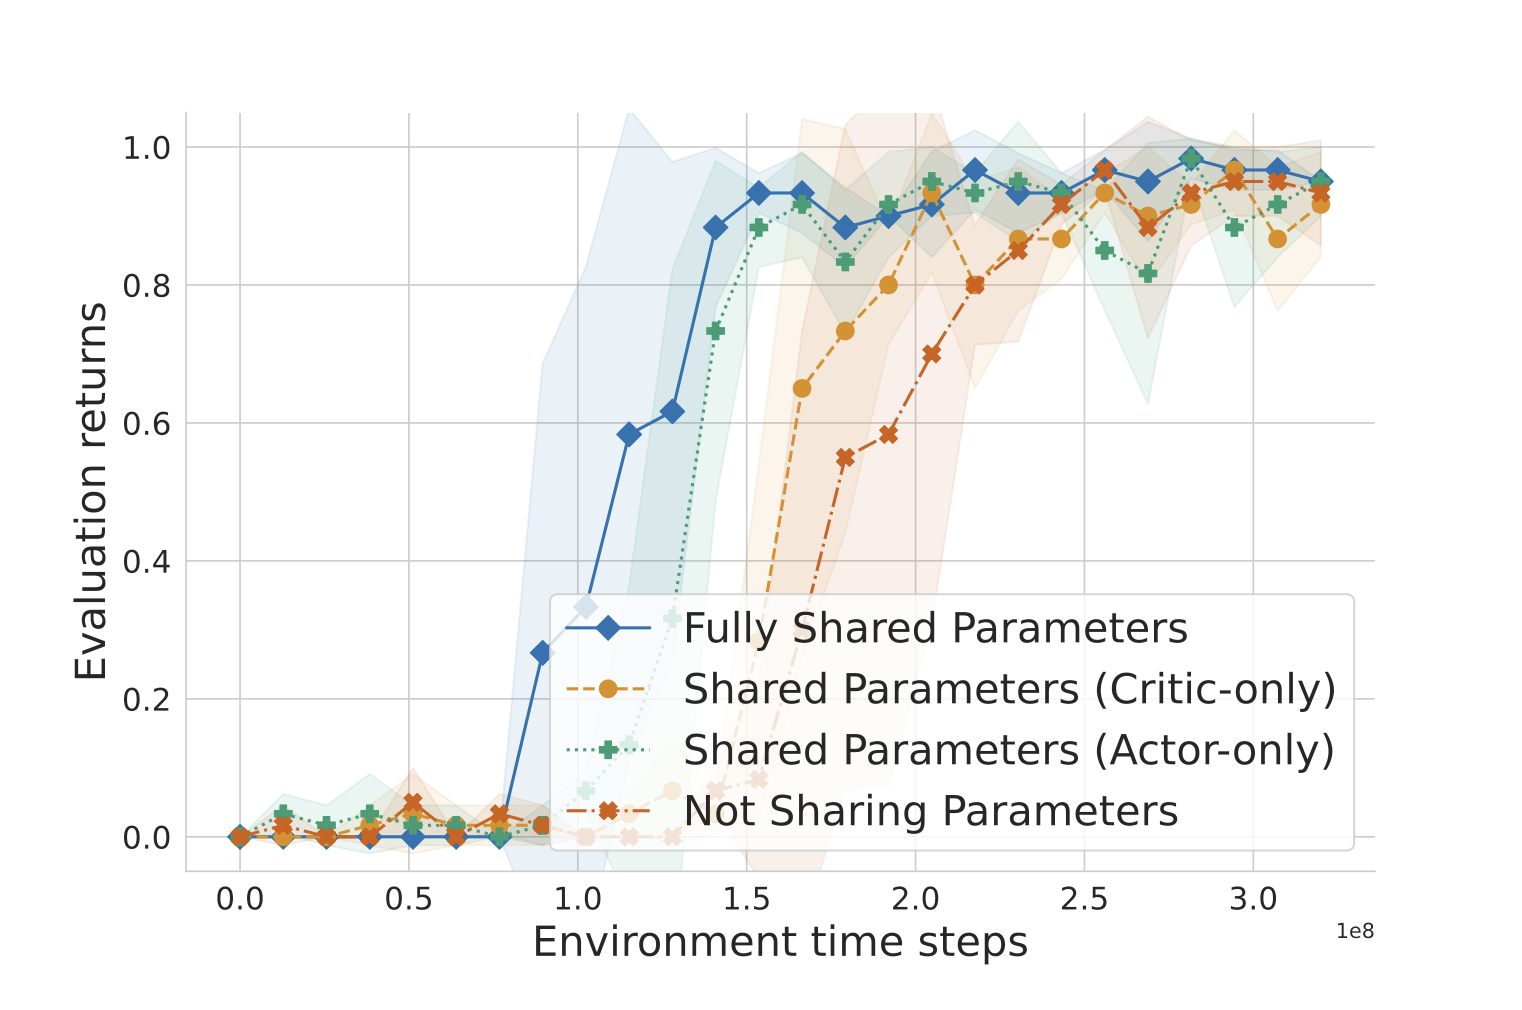
\includegraphics[width=0.8\textwidth, height=0.62\textheight,
        keepaspectratio]{media/lbf_param_share.png}

    \vspace{0.3em}
    {\small Learning curves for independent A2C with and without
    parameter sharing on level-based foraging.
    Figure taken from \cite{albrecht2024multi}.}
\end{frame}


% Subsection --- Experience sharing
\subsection{Experience Sharing}
\begin{frame}
    \frametitle{Experience sharing}
    So, how do we exploit homogeneity properties in environments with weakly homogeneous agents?

    Agents may need to learn different policies but that doesn't mean that they cannot use experiences of each other.

    How?

\end{frame}


\begin{frame}
\frametitle{Independent vs. Shared Replay Buffers}
\centering
\begin{adjustbox}{max width=0.98\textwidth,max height=0.72\textheight}
\begin{tikzpicture}[
    card/.style={
        rectangle, rounded corners=2pt,
        draw=cardborder, thick,
        fill=cardfill,
        minimum width=2.6cm, minimum height=0.45cm,
        font=\scriptsize, align=center
    },
    shadowcard/.style={
        rectangle, rounded corners=2pt,
        draw=cardborder!50, thin,
        fill=cardfill!60!white,
        minimum width=2.6cm, minimum height=0.45cm
    },
    container/.style={
        rectangle, rounded corners=6pt,
        draw=black, thick,
        minimum width=3.0cm
    },
    sharedcontainer/.style={
        rectangle, rounded corners=6pt,
        draw=blue!60!black, very thick,
        fill=blue!3,
        minimum width=3.2cm
    },
    title/.style={font=\bfseries\large, align=center},
    dots/.style={font=\large},
    caption/.style={align=center, font=\small, text width=3.6cm}
]

% =====================================================
% LEFT: independent replay buffers
% =====================================================
\node[title] at (-4.5,3.5) {Independent replay buffers};

% ---- Buffer 1 (Agent 1) ----
\node[shadowcard] at (-4.3,2.56) {};
\node[shadowcard] at (-4.4,2.49) {};
\node[card] (b1t) at (-4.5,2.42) {$(s_1,a_1,r_1,s_1')$};
\node[dots] (b1d) at (-4.5,1.9) {$\vdots$};
\node[card] (b1b) at (-4.5,1.38) {$(s_2,a_2,r_2,s_2')$};
\begin{pgfonlayer}{background}
\node[container, fit=(b1t)(b1b), inner sep=6pt] (buf1) {};
\end{pgfonlayer}
\node[font=\small] at (buf1.west) [anchor=east, xshift=-4pt] {Agent 1};

% ---- Buffer 2 (Agent 2) ----
\node[shadowcard] at (-4.3,0.16) {};
\node[shadowcard] at (-4.4,0.09) {};
\node[card] (b2t) at (-4.5,0.02) {$(s_1,a_1,r_1,s_1')$};
\node[dots] (b2d) at (-4.5,-0.5) {$\vdots$};
\node[card] (b2b) at (-4.5,-1.02) {$(s_2,a_2,r_2,s_2')$};
\begin{pgfonlayer}{background}
\node[container, fit=(b2t)(b2b), inner sep=6pt] (buf2) {};
\end{pgfonlayer}
\node[font=\small] at (buf2.west) [anchor=east, xshift=-4pt] {Agent 2};

\node[dots] at (-4.5,-1.9) {$\vdots$};

% ---- Buffer 3 (Agent K) ----
\node[shadowcard] at (-4.3,-2.64) {};
\node[shadowcard] at (-4.4,-2.71) {};
\node[card] (b3t) at (-4.5,-2.78) {$(s_1,a_1,r_1,s_1')$};
\node[dots] (b3d) at (-4.5,-3.3) {$\vdots$};
\node[card] (b3b) at (-4.5,-3.82) {$(s_2,a_2,r_2,s_2')$};
\begin{pgfonlayer}{background}
\node[container, fit=(b3t)(b3b), inner sep=6pt] (buf3) {};
\end{pgfonlayer}
\node[font=\small] at (buf3.west) [anchor=east, xshift=-4pt] {Agent $K$};

\node[caption] at (-4.5,-4.9) {Each agent stores transitions in its own replay buffer};

% =====================================================
% RIGHT: shared replay buffer
% =====================================================
\node[title] at (4.3,3.5) {Shared replay buffer};

\node[shadowcard] at (4.4,1.76) {};
\node[shadowcard] at (4.35,1.69) {};
\node[card] (s1) at (4.3,1.62) {$(s_1,a_1,r_1,s_1')$};
\node[card] (s2) at (4.3,1.10) {$(s_2,a_2,r_2,s_2')$};
\node[dots]      at (4.3,0.60) {$\vdots$};
\node[card] (s3) at (4.3,0.10) {$(s_3,a_3,r_3,s_3')$};
\node[card] (s4) at (4.3,-0.42) {$(s_4,a_4,r_4,s_4')$};
\begin{pgfonlayer}{background}
\node[sharedcontainer, fit=(s1)(s4), inner sep=7pt] (shared) {};
\end{pgfonlayer}

\node[caption] at (4.3,-1.8) {All agents store transitions in one shared replay buffer};

\end{tikzpicture}
\end{adjustbox}
\end{frame}

% =========================================================
% (5) Caveat: only off-policy + bridge to importance sampling
% =========================================================
\begin{frame}{Caveat of experience sharing}

\begin{itemize}
    \item The shared replay buffer works because DQN is
    \textbf{off-policy}: it can learn from transitions generated by
    \emph{any} policy --- including other agents' policies.
    \item \textbf{On-policy} algorithms such as A2C or PPO require
    trajectories sampled from the \emph{current} policy being
    optimized $\Rightarrow$ we cannot directly feed them
    other agents' experience.
\end{itemize}

\vspace{0.8em}
\centering
So, is experience sharing off-limits for on-policy methods?

\vspace{0.3em}
\textbf{No} --- Shared Experience Actor-Critic (SEAC) uses
\emph{importance sampling} to correct for transitions collected by
other agents.

\end{frame}

% =========================================================
% (5) Recap: importance sampling (Sutton & Barto)
% =========================================================
\begin{frame}
\frametitle{Recap: Importance Sampling~\cite{sutton2018reinforcement}}

\begin{block}{Estimating expectations under a different distribution}
We can estimate an expectation under a \emph{target} policy $\pi$ using
samples generated by a \emph{behavior} policy $\pi_\beta$ by re-weighting
each sample with the \textbf{importance sampling ratio}:
\[
\expect_{a \sim \pi}\!\left[ f(a) \right]
=
\expect_{a \sim \pi_\beta}\!\left[
\frac{\pi(a)}{\pi_\beta(a)} \, f(a)
\right]
\]
\end{block}

\vspace{0.4em}
Applied to the policy gradient, the loss for off-policy optimization
from a behavioral policy $\pi_\beta$ becomes:
\begin{center}
\adjustbox{max width=\linewidth}{$
\mathcal{L}(\phi)
=
-
\frac{\pi(a^t \mid h^t; \phi)}{\pi_{\beta}(a^t \mid h^t)}
\left(
    r^t + \gamma V(h^{t+1}; \theta) - V(h^t; \theta)
\right)
\log \pi(a^t \mid h^t; \phi)
$}
\end{center}

\vspace{0.4em}
\centering
$\Rightarrow$ Exactly the correction SEAC needs to reuse
\emph{other agents'} on-policy trajectories.

\end{frame}

% =========================================================
% (6) SEAC with colored loss terms
% =========================================================
\begin{frame}
    \frametitle{SEAC~\cite{albrecht2024multi}}
    \begin{center}
    \adjustbox{max width=\linewidth}{$
\begin{aligned}
\mathcal{L}(\phi_i)
&=
{\color{seacown}
-\left(
    r_i^t
    + \gamma V(h_i^{t+1}; \theta_i)
    - V(h_i^t; \theta_i)
\right)
\log \pi(a_i^t \mid h_i^t; \phi_i)
}
\\[0.5em]
&\quad
{\color{seacshared}
-\lambda
\sum_{k \ne i}
\underbrace{
\frac{
    \pi(a_k^t \mid h_k^t; \phi_i)
}{
    \pi(a_k^t \mid h_k^t; \phi_k)
}
}_{\text{importance sampling}}
\left(
    r_k^t
    + \gamma V(h_k^{t+1}; \theta_i)
    - V(h_k^t; \theta_i)
\right)
\log \pi(a_k^t \mid h_k^t; \phi_i)
}
\end{aligned}
$}
\end{center}

\vspace{0.8em}
\begin{itemize}
    \item {\color{seacown} \textbf{Own experience:}} the standard
    on-policy actor-critic loss of agent $i$.
    \item {\color{seacshared} \textbf{Shared experience:}} trajectories
    of all other agents $k \ne i$, treated as off-policy data and
    corrected via importance sampling --- this is what makes experience
    sharing possible in an \emph{on-policy} setting.
\end{itemize}
\end{frame}